%% --------------------%% --------------------%% --------------------%% --------------------%% ------------------------

1.A  Converting from Decimal to Binary
1.B  Converting from Decimal to Hexadecimal
1.C  Converting from Binary to Decimal
1.D  Converting from Hexadecimal to Decimal
1.E  Binary Addition
1.F  Binary Subtraction

%% --------------------%% --------------------%% --------------------%% --------------------%% ------------------------

2.A  Membership Tables
2.B  Venn Diagrams
2.C  Set differences and symmetric difference
2.D  
2.E



\end{enumerate}


% \item The Fibonacci sequence $f_n$ is defined recursively by the rule
%   \begin{equation*}
%     \begin{cases}
%       f_0&=0\\
%       f_1&=1\\
%       f_n&=a_{n-1}+a_{n-2}
%     \end{cases}
%   \end{equation*}

%   \begin{enumerate}
%   \item
%     Write a program to evaluate the Fibonacci sequence and hence evaluate $f_{50}$.
%   \item
%     Let the sequence $g_n$ be defined as the ratio
%     \begin{equation*}
%       g_n = \frac{f_{n+1}}{f_n}
%     \end{equation*}
%     Write a program to evaluate the first $50$ terms of the sequence $g_n$.
%   \item
%     Assumming that the sequence $g_n$ has a limit $\phi$, find this limit.
%   \end{enumerate}


\subsection*{Floating Point Notation}
(Demonstration on white board)



In mathematics, the cardinality of a set is a measure of the "number of elements of the set". For example, the set A = {2, 4, 6} contains 3 elements, and therefore A has a cardinality of 3.

\section{Set Theory}
\begin{enumerate}
\item The Universal Set $\mathcal{U}$
\item Union
\item Intersection
\item Set Difference
\item Relative Difference
\end{enumerate}



DE Muorgan's Laws (Useful for Propositions)

membership tables

proof by truth tables
AND
OR
NOT
Set difference
symmetric difference



\newpage


Harmonic Mean

\[ H_x = \frac{ n }{ \frac{ 1 }{ x_1 } + \frac{ 1 }{ x_2 } + \cdots + \frac{ 1 }{ x_n } } \]

2,4,6,8
> 1/mean(1/a)
[1] 3.84
> 1/a
[1] 0.5000000 0.2500000 0.1666667 0.1250000
> sum(1/a)
[1] 1.041667
> sum(1/a)*24
[1] 25
> 96/25
[1] 3.84



%----------------------------------------%

\subsection{Functions}
Evaluate $f(6)$ 


\[ f(x) = \lfloor \frac{x+1}{2} \rfloor \]


\[ f(6) = \lfloor \frac{\boldsymbol{6}+1}{2}\rfloor = \lfloor  \frac{7}{2}\rfloor\]


\[  \lfloor 3.5 \rfloor  = 3  \]


%----------------------------------------%

\subsection{Functions}
Evaluate $f(-6)$ 


\[ f(x) = \lfloor \frac{x+1}{2} \rfloor \]


\[ f(6) = \lfloor \frac{\boldsymbol{-6}+1}{2}\rfloor = \lfloor  \frac{-5}{2}\rfloor\]


\[  \lfloor -2.5 \rfloor  = -3  \]






% http://www.textbooksonline.tn.nic.in/books/12/std12-bm-em-1.pdf



%-----------------------------------%

\subsection{Discrete Maths : Relations}

%% %% - \vspace{-2cm}
\textbf{Example}
\begin{itemize}
\item Let $A = \{2, 3, 4, 6\}$ and $B = \{4, 6, 9\}$
\item Let R be the relation from A to B defined by \textit{\textbf{xRy}} if $x$
divides $y$ exactly.
\end{itemize}


%-----------------------------------%

\subsection{Discrete Maths : Relations}

%% %% - \vspace{-0.7cm}
\textbf{Example}
\begin{itemize}

\item Let $A = \{2, 3, 4, 6\}$ and $B = \{4, 6, 9\}$
\item Let R be the relation from A to B defined by \textit{\textbf{xRy}} if $x$
divides $y$ exactly.
\item  Then
\[R = {(2, 4), (2, 6), (3, 6), (3, 9), (4, 4), (6, 6)}\]
\end{itemize}



%------------------------------------------------------------------------%
\section{Arrow Diagrams}

\begin{itemize}

\item Domain
\item Co-Domain
\item Range
\end{itemize}
\[  f(x) : \mbox{Domain} \rightarrow \mbox{Co-Domain} \]
\[  f(x) : \mathbb{R} \rightarrow \mathbb{R} \]
%----------------------------------------------------------- %
\newpage
\subsection*{Polynomial Functions (4.1.5)}

\begin{itemize}
\item[Constants] $(P_0)$
\item[Linear Functions] $(P_1)$
\item[Quadratic Functions] $(P_2)$
\item[Cubic Functions] $(P_3)$
\end{itemize}


\subsection*{Equality of Functions (4.1.6)}
\[f(x) = g(x) \]




%------------------------------------------------------%
\subsection{Exercise} 
$h(x): \mathbb{R} \rightarrow \mathbb{R}$ 
$g(x): \mathbb{R} \rightarrow \mathbb{R}$

\[f(x) = sqrt(x)\]
\[g(x) = \sqrt{3}{x+2}\]
\[h(x) = 2^x\]

\begin{itemize}
\item Is the function $h(x)$ an \textit{onto} function?
\item determine the inverse function of $h(x)$ and $g(x)$
\item Simplify the following function.
\[ j(x) = \mbox{log}_4(h(6x))\]
\end{itemize}
%--------------------------------------------%
\subsection{Onto Functions}
Definition: If every element in the co-domain of the function has an ancestor, the function is said to be "onto".
An onto function has the property that the domain is equal to the co-domain.


\textbf{Example 4.26 Page 53}

%------------------------------------------------------------------------%
\section{\textit{One-to-One} Functions and \textit{Onto} Functions}

\subsection{Invertible Functions}
\begin{itemize}
\item One-to-One Function
\item Onto Function
\end{itemize}

Onto Functions : Range and Co-Domain are equivalent

\subsection{Inverting a Function}

\begin{itemize}
\item[$\bullet$] You are given $f(x)$ in terms of $x$
\item[$\bullet$] Re-arrange the equation so that $x$ is given in terms of $f(x)$
\item[$\bullet$] Replace $x$ with $f^{-1}(x)$ and $f(x)$ with $x$
\end{itemize}

\subsubsection{Example}
\begin{itemize}
\item[$\bullet$]Determine the inverse function of $f(x)$. Re-arrange the equation so that $x$ is given in terms of $f(x)$
\[  f(x): \mathbb{R} \rightarrow \mathbb{R}  \mbox{   } f(x)  = \sqrt{x+1} \]
\item[$\bullet$] Square both sides of the equation.
\[[f(x)]^2 = x+1 \]
\item[$\bullet$] Subtract 1 from both sides of the equation. We have the equation written in terms of x.
\[f(x)^2-1 = x \]
\item[$\bullet$] Replace $x$ with $f^{-1}(x)$ and $f(x)$ with $x$
\[x^2-1 = f^{-1}(x) \]
\item[$\bullet$] 
Re-arrange equation and specify domain and co-domain.
\[ f(x): \mathbb{R} \rightarrow \mathbb{R}  \mbox{   }  f^{-1}(x) = x^2-1  \]
\end{itemize}
% \[ f(x)  = \sqrt{x+1} \]
% \[f(x)^2 = x+1 \]
% \[f(x)^2-1 = x \]
% \[x^2-1 = f^{-1}(x) \]
\newpage
\section{Big O-Notation}

%------------------------------------------------------------------------%
% Section 4 Functions
% http://doc.gold.ac.uk/~maa01km/solutions/tut4sol.pdf
\begin{itemize}
\item[(b)] Let $S$ be the set of all 4 bit binary strings. 

The function $f : S \rightarrow \mathbb{Z}$
is defined by the rule:
\[f(x) = \mbox{the number of zeros in x}\]
for each binary string $x \in S$.\\
Find:
\begin{enumerate}
\item the number of elements in the domain
\item $f(1000)$
\item the set of pre-images of 1
\item the range of $f$.
\end{enumerate}
\item[(c)]
\end{itemize}
\newpage
\begin{itemize}
\item[4.a] $ \lfloor x - y \rfloor = \lfloor x \rfloor - \lfloor y \rfloor$
\item[4.b]
\item[4.c]
\end{itemize}
\newpage
%------------------------------------------------------------------------%
\section{Section 4 Functions}

\subsection{Invertible Functions}
A function is invertible if it fulfils two criteria
\begin{itemize}
\item The function is \textbf{\textit{onto}},
\item The function is \textbf{\textit{one-to-one}}.
\end{itemize}

State the conditions to be satisfied by a function
$f : X \leftarrow Y$ for it to have an inverse function
$f^{-1} : Y \leftarrow X$.
%---------------------------------------------------------%

$\lceil \frac{x^2+1}{4} \rceil$
where $f : A \rightarrow \textbf{Z}$
\begin{itemize}
\item[(i)] Find $f(4)$ and the ancestors of 3.
\item[(ii)] Find the range of $f$.
\item[(iii)] Is f invertible? Justify your answer
\end{itemize}

Given $f : \textbf{R} \rightarrow \textbf{R}$ where f(x) =3x-1,define fully
the inverse of the function f ,i.e.$f^{-1}$. 
State the value of $f^{-1}(2)$



\section{Laws of Exponents}
Here are the Laws (explanations follow):

LawExample
x1 = x61 = 6
x0 = 170 = 1
x-1 = 1/x4-1 = 1/4
xmxn = xm+nx2x3 = x2+3 = x5
xm/xn = xm-nx6/x2 = x6-2 = x4
(xm)n = xmn(x2)3 = x2×3 = x6
(xy)n = xnyn(xy)3 = x3y3
(x/y)n = xn/yn(x/y)2 = x2 / y2
x-n = 1/xnx-3 = 1/x3
%--------------------------------------------------%
Z Score
\[ Z = \frac{X - \mu}{\sigma} \]
%--------------------------------------------------%




%-------------------------------------------------------%


%% --------------------
\subsection{Exercises}

Showing your workings, use the rules of indices and logarithms to give the following two expression in their simplest form.
\bigskip
\begin{itemize}
\item \textbf{Exercise 1}
\[ 4 \cdot 2^x - 2^{x+1} \]
\item \textbf{Exercise 2}
\[  \frac{\mbox{ln}(2) + \mbox{ln}(2^2) + \mbox{ln}(2^3)  + \mbox{ln}(2^4) + \mbox{ln}(2^5)  }  {\mbox{ln}(4)}  \]
\end{itemize}
%% --------------------

%-------------------------------------------------------%
%% --------------------
\subsection{Exercise 1}

\[ 4 \cdot 2^x - 2^{x+1} \]

\textbf{Remarks:}\\
\textit{(looking at the second term)}
\begin{itemize}
\item[1] Using the following rule
\[ a^b \cdot a^c = a^{(b+c)}  \] 
\item[2] Using this rule in reverse we can say
\[ 2^{x+1} = 2^x \cdot 2^1  = 2\cdot (2^x) \] 
\end{itemize}
\[ 4 \cdot 2^x - 2^{x+1} \mbox{   } = \mbox{   } (4 \cdot 2^x) -  (2\cdot 2^{x}) \]
%% --------------------

%-------------------------------------------------------%
%% --------------------
\subsection{Exercise 1}

%% %% - \vspace{-0.9cm}

\textbf{Remarks:}
\begin{itemize}
\item[3] This expression is in the form 
\[ (a  \cdot b ) - ( c  \cdot b) \]
which can be re-expressed as follows 
\[ (a - c\sqrt{b} )  \cdot b \]
\end{itemize}
\[ (4 \cdot 2^x) -  (2\cdot 2^{x}) = (4-2)  \cdot 2^{x} \]
\[   = 2 \cdot 2^x = 2^{x+1}\]
%% --------------------
%-------------------------------------------------------%

%% --------------------
\subsection{Exercise 2}


\[  \frac{\mbox{ln}(2) + \mbox{ln}(2^2) + \mbox{ln}(2^3)  + \mbox{ln}(2^4) + \mbox{ln}(2^5)  }  {\mbox{ln}(4)}  \]
Useful Rule of Logarithms
\[  \mbox{ln}(a^b)  = b\cdot \mbox{ln}(a)  \]
\[  \frac{\mbox{ln}(2) + 2 \cdot \mbox{ln}(2) + 3 \cdot\mbox{ln}(2)  + 4 \cdot \mbox{ln}(2) + 5 \cdot \mbox{ln}(2)  }  {\mbox{ln}(4)}  \]
%% --------------------
%--------------------------------------%
%% --------------------
\subsection{Exercise 2}

Adding up all the terms in the numerator

\[  \frac{1\cdot\mbox{ln}(2) + 2 \cdot \mbox{ln}(2) + 3 \cdot\mbox{ln}(2)  + 4 \cdot \mbox{ln}(2) + 5 \cdot \mbox{ln}(2)  }  {\mbox{ln}(4)} \]  \[= \frac{15 \cdot \mbox{ln}(2) }{\mbox{ln}(4)} \]


%% --------------------

%--------------------------------------%
%% --------------------
\subsection{Exercise 2}

Our expression has now simplified to 
\[\frac{15 \cdot \mbox{ln}(2) }{\mbox{ln}(4)} \]

We can simplify the denominator too

\[ \mbox{ln}(4) =  \mbox{ln}(2^2) = 2 \cdot \mbox{ln}(2) \]


%% --------------------

%--------------------------------------%
%% --------------------
\subsection{Exercise 2}

Our expression has now simplified to 
\[\frac{15 \cdot \mbox{ln}(2) }{\mbox{ln}(4)} = \frac{15 \cdot \mbox{ln}(2) }{2 \cdot \mbox{ln}(2)} \]

We can divide above and below by $\mbox{ln}(2)$ to get our final answer


\[ \frac{15 \cdot \mbox{ln}(2) }{2 \cdot \mbox{ln}(2)} = \frac{15}{2} = 7.5 \]

%% --------------------

%% --------------------
%-----------------------------------------------------%
\section*{Prepositional Logic}


%-------------------------------------------------------------------------%
\newpage
\section{Section 3 Logic}

\begin{center}
\begin{tabular}{|c|c|c|c|c|}
\hline
p & q & $p \vee q$ & $q \wedge p$ & $p \otimes q$ \\
\hline
0 & 0 & 0 & 0 & 0 \\
0 & 1 & 1 & 0 & 1\\
1 & 0 & 1 & 0 & 1 \\
1 & 1 & 1 & 1 & 0\\
\hline
\end{tabular}
\end{center}
%---------------------------------------------------------%
\section{Conditional Connectives}
Construct the truth table for the proposition $p \rightarrow q$.

\begin{center}
\begin{tabular}{|c|c|c|c|}
\hline
p & q & $p \rightarrow q$ & $q \rightarrow p$ \\
\hline
0 & 0 & 1& 1 \\
0 & 1 & 1 & 0 \\
1 & 0 & 0 & 1 \\
1 & 1 & 1 & 1 \\
\hline
\end{tabular}
\end{center}


\subsection*{Question 4}
%2001 Question 4
\begin{center}
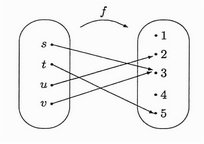
\includegraphics[scale=0.55]{HibCollArrow.jpg}
\end{center}




\subsection*{Question 10}

(a) Given the following adjacency matrices A and B where
%A =
%
%1 0 1
%0 1 2
%1 2 0
%
% ,B =
%
%1 2 0
%2 0 1
%0 1 1

%MAKE NO




\subsection*{Dice Rolls}
Consider rolls of a die. What is the universal set?

\[ \mathcal{U} = \{1,2,3,4,5,6\} \]

%--------------------------------------%

\subsection*{symbols}
$\varnothing$,
$\forall$,
$\in$,
$\notin$,
$\cup$

\chapter{Sequences and Series, and Proof by Induction}
\section{Sequence and Series and Proof by Induction}


\[\sum (n^2) \]






%------------------------------------------------------------------------- %
\section{Revision Questions}



\[  2^ 4 = 2 \times 2 \times 2 \times 2 = 16 \]

\[  5^ 3 = 5 \times 5 \times 5 =125 \]

\subsubsection{Special Cases}

Anything to the power of zero is always 1

\[  X^ 0 = 1 \mbox{ for all values of X} \]

Sometimes the power is a negative number.

\[  X^{-Y} = { 1 \over X^Y}  \]

Example 
\[  2^{-3} = { 1 \over 2^3} = { 1 \over 8}  \]


%====================================== %
\newpage
\begin{center}
\huge{Mathematics for Computing}\\
{ Session 2 : Set Theory}
\end{center}



%-------------------------- %
%-------------------------- %
%Section 5 Graph Theory

\section*{Equivalence Relations}

%%%%%%%%%%%%%%%%%%%%%%%%%%%%%%%%%%%%%%%%%%%%%%%%%%%%%%%%%%%%%%%%5

\subsection*{Session 04:Functions}
\begin{itemize}
\item Definitions
\end{itemize}

\begin{itemize}
\item[Domain]
\item[Co-domain]
\item[Image]
\item[Ancestor]
\item[Range]
\end{itemize}

\subsection*{Part A : Functions}
Given a real number $x$, say how the floor of x  $\lfloor x \rfloor$ is defined.
\begin{itemize}
\item[(i)] Find the values of $\lfloor 2.97 \rfloor$ and $\lfloor -2.97 \rfloor$.
\item[(ii)] Find an example of a real number $x$ such that $\lfloor 2x \rfloor  \neq 2\lfloor x \rfloor$, justifying your answer.
\end{itemize}



\subsection*{Floor and Ceiling Function (4.1.4)}
\subsection*{Polynomial Functions (4.1.5)}

\begin{itemize}
\item[Constants] $(P_0)$
\item[Linear Functions] $(P_1)$
\item[Quadratic Functions] $(P_2)$
\item[Cubic Functions] $(P_3)$
\end{itemize}


\subsection*{Equality of Functions (4.1.6)}
\[f(x) = g(x) \]



\subsection*{One-to-One Functions (4.2.3)}
$f(x)$, must be \emph{One-to-One} and \emph{Onto}



\subsection*{Exponential and Logarithmic Functions (4.3)}

The Laws of Logarithms
\begin{itemize}
\item
\item $log_b(x^y) = y \times log_b(x)$
\item
\item
\end{itemize}
%================================================================== %


\section*{Functions}
\begin{itemize}
\item Domain of a Function
\item Range of a function
\item Inverse of a function
\end{itemize}
\begin{itemize}
\item one-one (surjective)
\item onto (bijective)
\end{itemize}
%------------------------------------------------%






\section{Video 7 : Numbers}


\begin{description}
\item[mantissa]
\item[abscissa]
\item[radix point]
\end{description}

\begin{itemize}
\item Number Systems
\item Set Theory
\item Function
\item 
\item Graph Theory
\end{itemize}



\begin{itemize}
\item Digraphs
\item Set Theory
\item Function
\item Probability
\item MAtrices
\end{itemize}



%\frametitle{(1.4.1) Decimal to Binary Conversion}
\begin{itemize}
\item Continuously divide the decimal number by 2.
\item Keep record of the remainder, either 0 or 1.
\item The sequence of remainders is the binary number required.
\end{itemize}

%------------------------------------------%

%\frametitle{Hexadecimal Numbers}
\begin{itemize}
\item Hex Characters $\{0,1,2,3,4,5,6,7,8,9,A,B,C,D,E,F\}$
\item 
\end{itemize}

%-------------------------------------%

%\frametitle{Relatiional Operators}
\begin{itemize}
\item $\neq$ Not Equal
\item < Less than
\item > greater than
\item $\geq$ greater than or equal to
\item $\leq$ Not Equal to
\end{itemize}

%------------------------------------------%

%\frametitle{Frame Name}
\begin{itemize}
\item Natural Numbers $\{1,2,3,4, \ldots\}$
\item Integers $\{\ldots,-2,-1,0,1,2,3,\ldots\}$
\item Rational Numbers e.g $4/7$ , $11/25$
\item Real Numbers Any number e.g. $3.1415$
\end{itemize}



%----------------------------------------------%

\begin{itemize}
\item Decmal Number Systesm
\begin{itemize}
\item Base 10
\end{itemize}

\item Binary Number Systems
\begin{itemize}
\item Base 2
\item allowable characters are {0.1} only
\end{itemize}
\item Base 16 Hexadecimal
\begin{itemize}
\item Use all of the decimal digits, in addition to 6 more A,B~,D,D,E,F
\end{itemize}
(where might you see this  - specifying colours RGB Numbers
\end{itemize}

%============================================================= %


%--------------------------------------------%

Computing a binary number

Useful
{
\begin{center}
\begin{tabular}{|c|c|}
\hline $2^0 = 1 $ & $2^4 = 16  $ \\ 
\hline $2^1 = 2 $ & $2^5 = 32$ \\ 
\hline $2^2 = 4 $ & $2^6 = 64$ \\ 
\hline $2^3 = 8 $ & $ 2^7 = 128$ \\ 
\hline 
\end{tabular} 
\end{center}
}



\end{document}
